\documentclass[12pt]{ctexart}
    %%% Document Settings %%%%
%\usepackage[utf8]{inputenc}

\usepackage[
    twoside,
    top=1in,
    bottom=0.75in,
    inner=0.5in,
    outer=0.5in,
]{geometry}
\pagestyle{myheadings}
\usepackage{minted}
\usepackage[dvipsnames,svgnames]{xcolor}

%%%% Additional Commands to Load %%%%
\usepackage{tcolorbox}
\tcbuselibrary{skins}
\tcbuselibrary{minted}
\usemintedstyle{lovelace}
%\usepackage{minted}
\usepackage{color}
\usepackage{tikz}
\usetikzlibrary{calc}
\usepackage{tabularx,colortbl}
\usepackage{amsfonts,amsmath,amssymb}
\usepackage{titling}
\usepackage{mathrsfs}
\usepackage{calc}
\usepackage{subcaption}

\usepackage{listings}
%\usepackage{newtxtext}
\usepackage[strict]{changepage} 
\usepackage{framed}
\definecolor{formalshade}{rgb}{0.95,0.95,1}
\usepackage{float}

%%%% Commands to Define Homework Boxes %%%%
%%%% Box Definition %%%%
\newtcolorbox{prob}[1]{
% Set box style
    sidebyside,
    sidebyside align=top,
% Dimensions and layout
    width=\textwidth,
    toptitle=2.5pt,
    bottomtitle=2.5pt,
    righthand width=0.20\textwidth,
% Coloring
    colbacktitle=gray!30,
    coltitle=black,
    colback=white,
    colframe=black,
% Title formatting
    title={
        #1 \hfill Grade:\phantom{WWWW}
    },
    fonttitle=\large\bfseries
}

%%%% Environment Definition %%%%
\newenvironment{problem}[1]{
    \begin{prob}{#1}
}
{
    \tcblower
    \centering
    \textit{\scriptsize\bfseries Faculty Comments}
    \vspace{\baselineskip}
    \end{prob}
}

\newenvironment{formal}{%
\def\FrameCommand{%
\hspace{1pt}%
{\color{DarkBlue}\vrule width 2pt}%
{\color{formalshade}\vrule width 4pt}%
\colorbox{formalshade}%
}%
\MakeFramed{\advance\hsize-\width\FrameRestore}%
\noindent\hspace{-4.55pt}% disable indenting first paragraph
\begin{adjustwidth}{}{7pt}%
\vspace{2pt}\vspace{2pt}%
}
{%
\vspace{2pt}\end{adjustwidth}\endMakeFramed%
}

    \title{特殊方程作业3}
    \author{地物2201班\ 杨曜堃}
    \date{\today}
%%% document
\begin{document}

% Format Running Header
    \markboth{\theauthor}{\thetitle}
    \maketitle
    \begin{description}
        \item[问题1] 采用分离变量法求解下列热传导方程定解问题$$
        \begin{cases}
            \dfrac{\partial u}{\partial t}=a^2\dfrac{\partial^2u}{\partial x^2},&\quad 0<x<1,\ t>0\\
            u|_{t=0}=4\sin \pi x& \\
            u|_{x=0}=0,\ u|_{x=1}=0& \\
        \end{cases}$$
    \end{description}
    % \begin{center}
    %     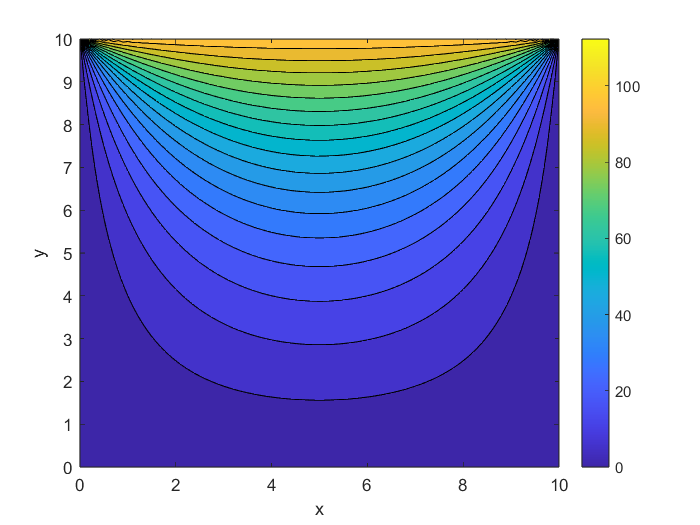
\includegraphics[width=16cm]{fig1.png}
    % \end{center}
    
    \begin{problem}{问题\#1}
        采用分离变量法,令$u(x,t)=X(x)T(t)$,代入偏微分方程得到
        $$
        \dfrac{X''(x)}{X(x)}=\dfrac{1}{a^2}\dfrac{T'(t)}{T(t)}=-\lambda
        $$
        $$
        \begin{cases}
            X''(x)+\lambda X(x)=0\\
            T'(t)+a^2\lambda T(t)
        \end{cases}
        $$
        利用本征值法,代入边界条件$$X(0)=X(1)=0$$,得到本征值和本征函数
        $$
        \lambda_n=(n\pi)^2,\ X_n(x)=\sin n\pi x,\ n=1,2,\cdots
        $$
        进一步求解一阶微分方程$\dfrac{T'(t)}{T(t)}=-(an\pi)^2$,方程两边对$t$积分得到
        $$
        \ln T_n(t)=-(an\pi)^2t+C
        $$
        $$
        T_n=C_ne^{-(an\pi)^2t}
        $$
        得到满足条件的一组特解
        $$
        u_n(x,t)=C_ne^{(-an\pi)^t}\sin n\pi x
        $$
        代入初始条件
        $$
        u|_{t=0}=\sum C_n\sin n\pi x=4\sin \pi x
        $$
        于是可以取$C_1=4$,得到定解问题的解
        $$
        u(x,t)=4e^{-(a\pi)^2t}\sin \pi x
        $$
    \end{problem}
\end{document}